% XCircuit output "osr8-raw.tex" for LaTeX input from osr8-raw.ps
\def\putbox#1#2#3#4{\makebox[0in][l]{\makebox[#1][l]{}\raisebox{\baselineskip}[0in][0in]{\raisebox{#2}[0in][0in]{\scalebox{#3}{#4}}}}}
\def\rightbox#1{\makebox[0in][r]{#1}}
\def\centbox#1{\makebox[0in]{#1}}
\def\topbox#1{\raisebox{-0.60\baselineskip}[0in][0in]{#1}}
\def\midbox#1{\raisebox{-0.20\baselineskip}[0in][0in]{#1}}
   \scalebox{1}{
   \normalsize
   \parbox{12.0469in}{
   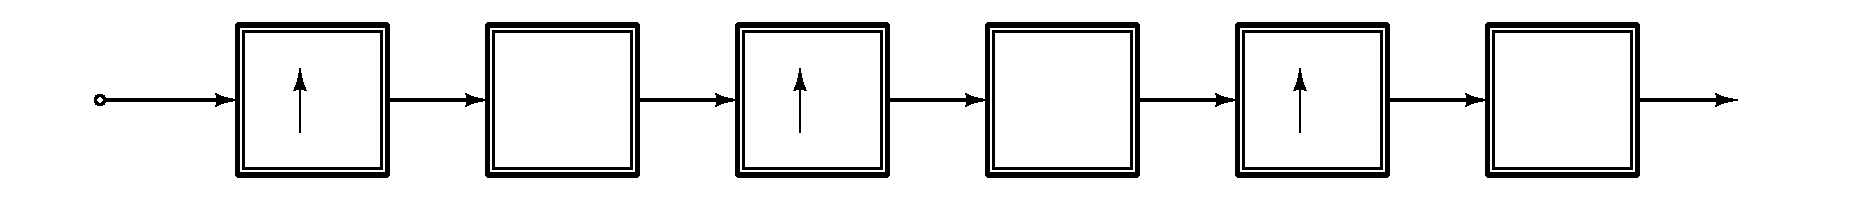
\includegraphics[scale=1]{osr8-raw}\\
   % translate x=1392 y=192 scale 0.38
   \putbox{0.81in}{0.72in}{1.80}{$f_s$}%
   \putbox{2.64in}{0.72in}{1.80}{$2f_s$}%
   \putbox{5.97in}{0.72in}{1.80}{$4f_s$}%
   \putbox{9.31in}{0.72in}{1.80}{$8f_s$}%
   \putbox{3.39in}{0.47in}{2}{$A(z)$}%
   \putbox{6.72in}{0.47in}{2}{$B(z)$}%
   \putbox{10.06in}{0.47in}{2}{$C(z)$}%
   \putbox{1.97in}{0.47in}{2}{$2$}%
   \putbox{5.31in}{0.47in}{2}{$2$}%
   \putbox{8.64in}{0.47in}{2}{$2$}%
   \putbox{0.06in}{0.56in}{1.80}{$x[n]$}%
   \putbox{11.56in}{0.56in}{1.80}{$y[n]$}%
   } % close 'parbox'
   } % close 'scalebox'
   \vspace{-\baselineskip} % this is not necessary, but looks better
